\newpage
\section{Instrumented Algorithm}
%
%----- why we need this section: what we offered is abstract and
%implementing it is not obvious
In section, we explain our detailed implementation of the consistency
preservation technique, defined in the previous section. Here, we use a
memoization technique to avoid redundencies in computations. The rules
presented in the previous section, made use of the notion of
dependencies and maintained consistent caches, by only checking if the
set of all dependencies for an effect is present in the cache or not (we
call this property the \emph{availability} of the effects).  
However, as an astute reader might have noticed, a naive implementation
of this idea, would result in a poor performance, when tracking the
dependencies for all effects. That is because, contracts can be
arbitrarily large in our system 
and they can contain closure of relation seeds, computing the
inverse of which can become very difficult, and is not reasonable to be
repeated before every execution. 


Now, we want to extend the notion of availability, to the \emph{degree of
availability}. By this extension, at every cache refresh, we can mark effects with a number,
representing \emph{how far} their dependencies are still missing from
the replica. This way we can capture the process in which the dependencies
become available, and avoind unnecessary redundant computations. 
\subsection{Definitions}

\subsection{Algorithms}
In this part, we will explain the outline of our algorithm using
an example. The formal operational semantics of this approach can be
found in appendix \ref{appendix:large_semantics}.

Let's assume we are given a contract $\psi=\forall (a,b). a
\xrightarrow{so;vis;so}b \Rightarrow a \xrightarrow{vis} b$ and now each
replica must maintain a cache, that is consistent according to this
contract. Replicas execute operations on this cache, and decide if a
newlly arrived remote effect, can enter the cache or not. 
A naive approach, would simply compute the set of all
dependencies after every effect arrival, and let it enter the cache if
they are all present at the replica. Here we propose our approach by
explaining the replica's behavior on certain events. 
\begin{itemize}
\item {\bf Effect Arrival:} When a new remote effect arrives to the
replica, it is simply added to the $\Pool$ and is given tag 3. This is
because the length of the given contract is 3, and this initial tag
means no dependency of this effect is checked so far.
\item {\bf Operation Submission: } Since the contract is a waiting
contract, the cache manager, must make sure that $so^{-1}$ of the
submitted operation is present in the cache, and if not block the
request for some time. After the dependencies become available in
the cache, the opertaion can go through and see all effects in the pool.
\item {\bf Cache Refresh: } The cache manager, must perform periodic
cache refreshes and move effects whose dependencies are present (i.e.
their availability degree is 1) to the cache. The effects are in fact
what will be shown to the operations.
\item {\bf Availability Refresh: } At this periodicstep, the
availability degree of effects, whose another layer of dependencies are
present, is decremented by one. For example, effects in the availability
set 3, whose $vis^{-1}$ is present in the pool, move the availaility set
2. Similarly, those whose $so^{-1}$ is present move to the availability
set 1.
\end{itemize}
\begin{figure}[t]
	\centering
	\setlength{\fboxsep}{6pt}%
	%\framebox[0.87\textwidth]{
	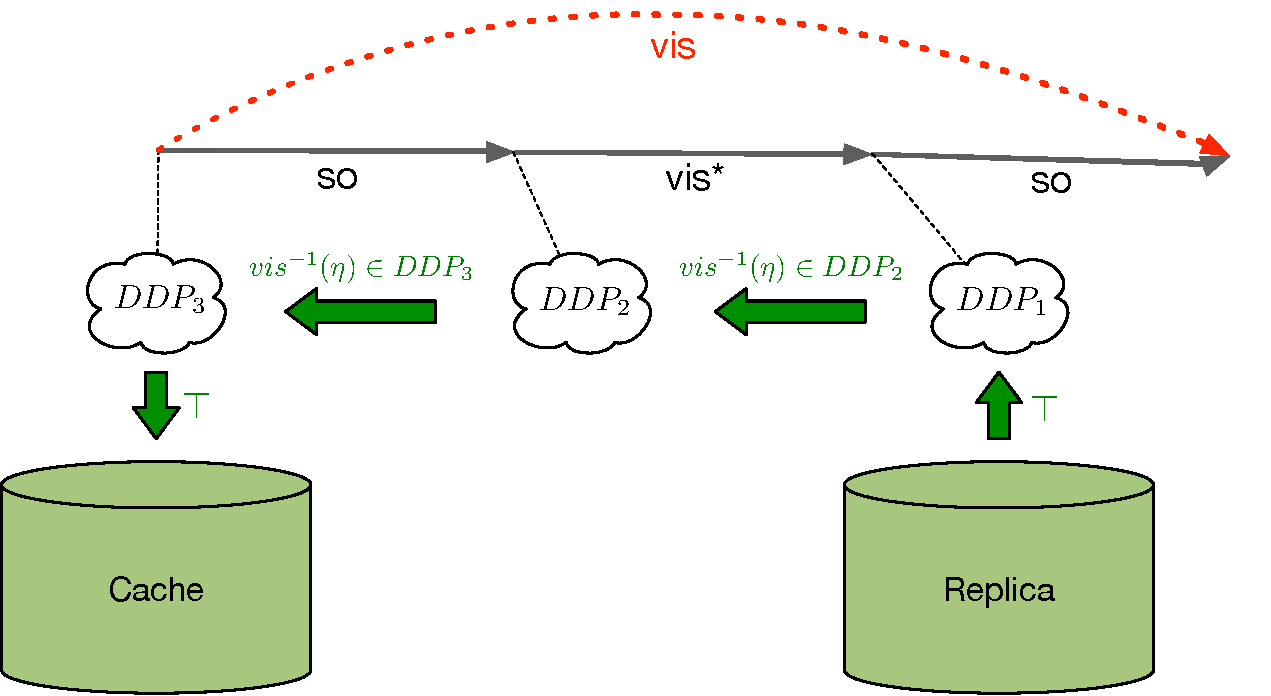
\includegraphics[scale =
	0.4]{Figures/Availability_deg.pdf}
	%}
	\\ 
	\hrulefill
\caption{Example of stepwise progress of effects before entering the
cache}
\label{fig:avail_deg}
\end{figure}

Note that, if one of the given relations, was a closure, we had to
change the last case so that at each step, the the dependencies were
looked for in the next availability set. For example, if the contract
was $\psi=\forall (a,b). a
\xrightarrow{so;vis^*;so}b \Rightarrow a \xrightarrow{vis} b$
an effect could move from availability set 3 to the availability set 2,
only if its $vis^{-1}$ was already included in the availability set 2
(as opposed to the normal case, were they should just be present in the
pool). This way, without the requirement to compute the inverse of the closur of
relation, which can potentially become very large, we can maintain the
required consistency level.










\newpage 
